\section{CKAN}
CKAN (Comprehensive Knowledge Archive Network) � un potente sistema DMS (Data Management System, ovvero un sistema di gestione dei dati) open source.
Esso ha lo scopo di rendere i dati accessibili permettendo la loro archiviazione e distribuzione attraverso una comoda interfaccia web che ne semplifica la pubblicazione, la condivisione, la ricerca e l'utilizzo.

Il funzionamento dell�architettura del sistema � mostrato in figura \ref{fig:ckan}.

\begin{figure}[htbp]
   \centering
   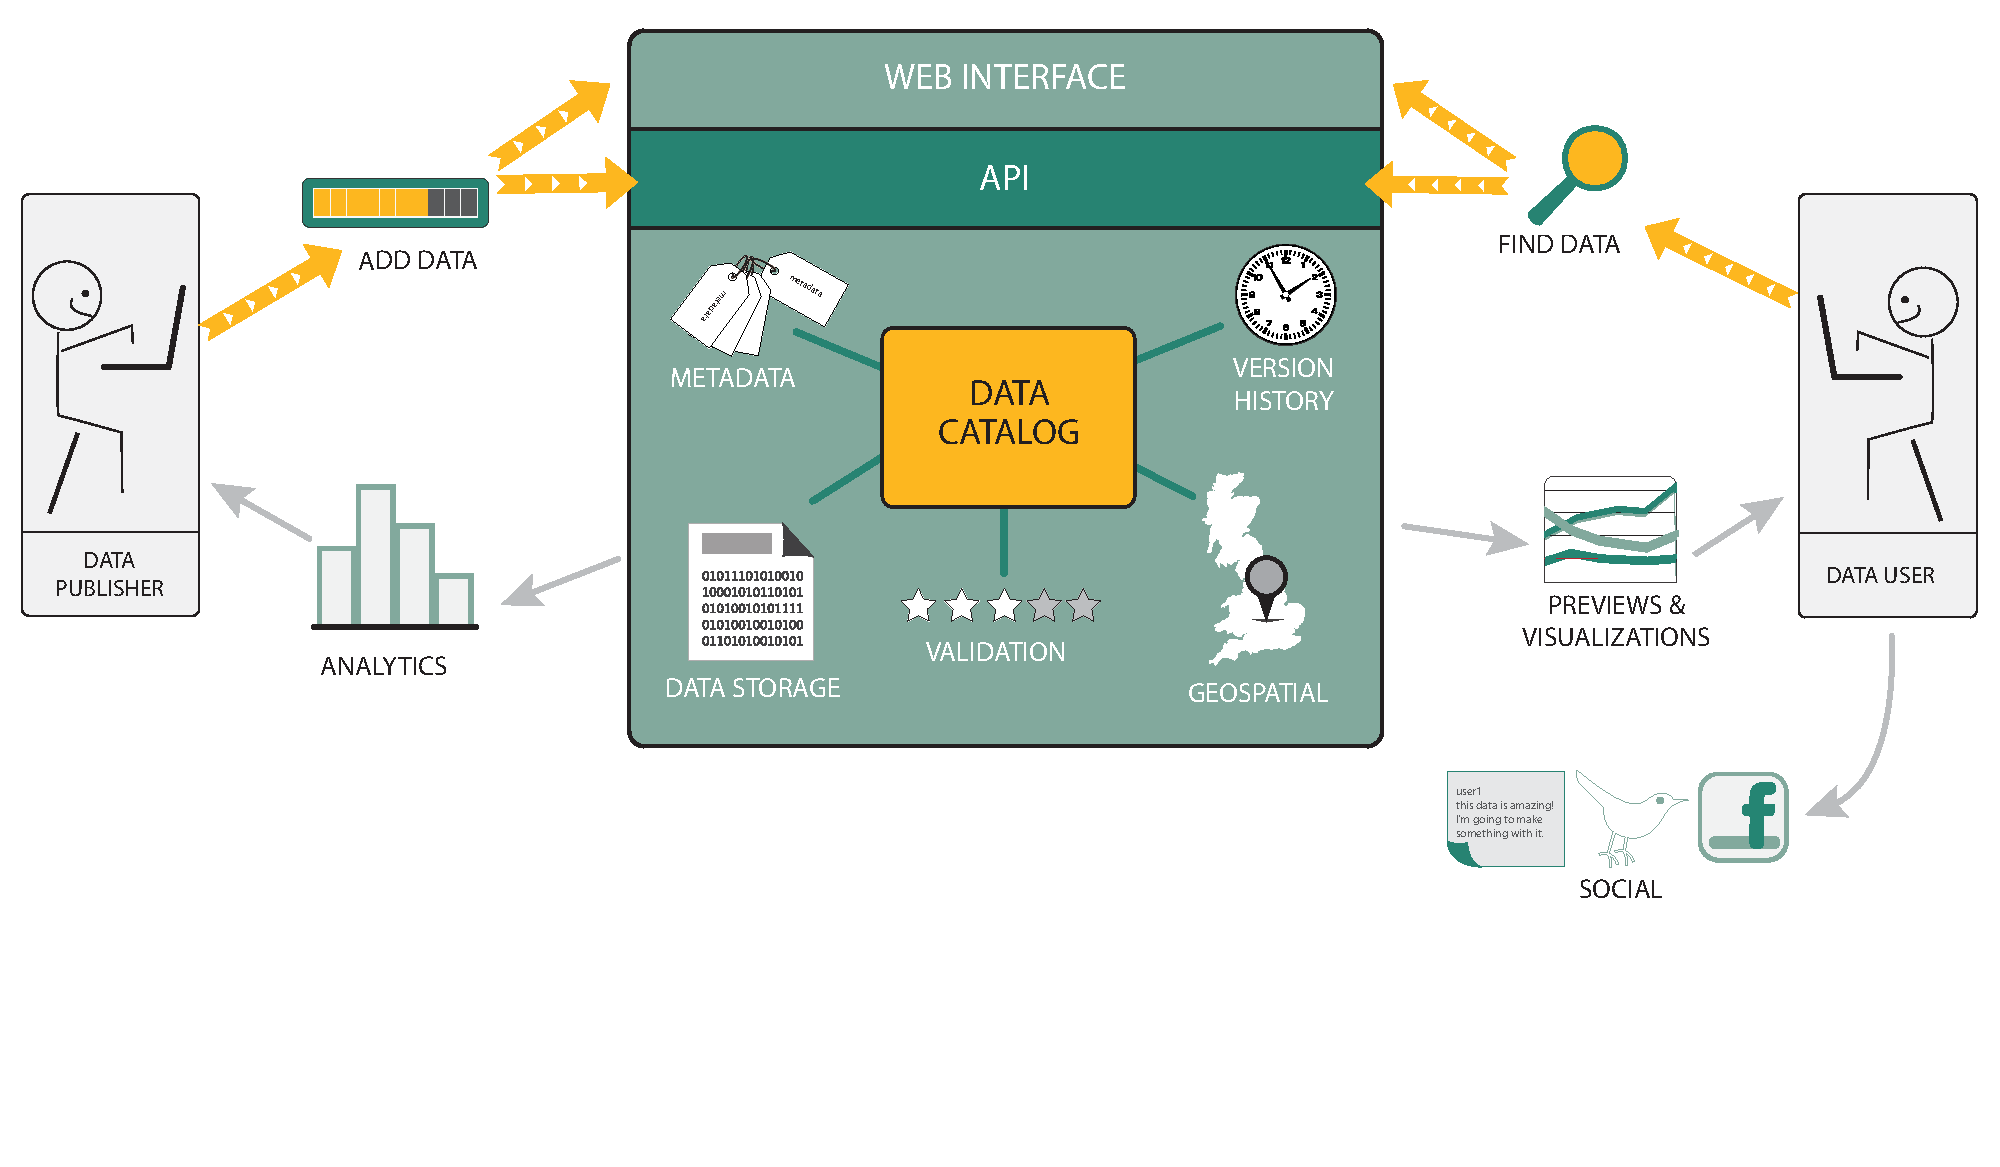
\includegraphics[scale=0.32,trim=0 4cm 0 0, clip=true]{img/ckan}
   \caption{Funzionamento Architettura CKAN}
   \label{fig:ckan}
\end{figure}

CKAN offre sia numerose API per gestire i dataset, che strumenti di visualizzazione che ne permettono una rapida anteprima.
La piattaforma supporta molto bene i dati in formato tabellare, siano essi semplici CSV o XLS, e la loro visualizzazione pu� essere fatta in semplice tabella, come grafico a punti o su una mappa in caso di dati geolocalizzati.

CKAN � rivolto ai data publishers, come governi, imprese o organizzazioni nazionali/regionali, che vogliono rendere disponibili e facilmente fruibili i propri dati. A ci� va aggiunta la possibilit� di integrare facilmente i cataloghi di altri portali sviluppati anch'essi in CKAN.

Il suo codice � mantenuto dalla Open Knowledge Foundation ed � utilizzato come piattaforma per gestire cataloghi pubblici da siti come \href{http://datahub.io/}{\texttt{datahub.io}}, \url{catalog.data.gov}, \url{data.gov.uk} e  \href{http://publicdata.eu/}{\texttt{PublicData.eu}}.

CKAN pu� essere installato gratuitamente su un server di propriet� dello stesso soggetto che intende pubblicare i dati, oppure � possibile acquistare il servizio di hosting dedicato gestito dallo stesso produttore di software (quindi in modalit� SaaS).

CKAN ha iniziato il suo sviluppo nel 2007, ma solo nel maggio 2010 � stata pubblicata la sua prima versione (1.0), alla quale sono seguiti aggiornamenti minori fino alla versione 1.8, che nel maggio 2013 � stata superata dalla nuova versione 2.0. Attualmente � in sviluppo la versione 2.2.
